\documentclass[]{elsarticle} %review=doublespace preprint=single 5p=2 column
%%% Begin My package additions %%%%%%%%%%%%%%%%%%%
\usepackage[hyphens]{url}

  \journal{Forest Ecology and Management} % Sets Journal name


\usepackage{lineno} % add
\providecommand{\tightlist}{%
  \setlength{\itemsep}{0pt}\setlength{\parskip}{0pt}}

\usepackage{graphicx}
\usepackage{booktabs} % book-quality tables
%%%%%%%%%%%%%%%% end my additions to header

\usepackage[T1]{fontenc}
\usepackage{lmodern}
\usepackage{amssymb,amsmath}
\usepackage{ifxetex,ifluatex}
\usepackage{fixltx2e} % provides \textsubscript
% use upquote if available, for straight quotes in verbatim environments
\IfFileExists{upquote.sty}{\usepackage{upquote}}{}
\ifnum 0\ifxetex 1\fi\ifluatex 1\fi=0 % if pdftex
  \usepackage[utf8]{inputenc}
\else % if luatex or xelatex
  \usepackage{fontspec}
  \ifxetex
    \usepackage{xltxtra,xunicode}
  \fi
  \defaultfontfeatures{Mapping=tex-text,Scale=MatchLowercase}
  \newcommand{\euro}{€}
\fi
% use microtype if available
\IfFileExists{microtype.sty}{\usepackage{microtype}}{}
\bibliographystyle{elsarticle-harv}
\usepackage{graphicx}
% We will generate all images so they have a width \maxwidth. This means
% that they will get their normal width if they fit onto the page, but
% are scaled down if they would overflow the margins.
\makeatletter
\def\maxwidth{\ifdim\Gin@nat@width>\linewidth\linewidth
\else\Gin@nat@width\fi}
\makeatother
\let\Oldincludegraphics\includegraphics
\renewcommand{\includegraphics}[1]{\Oldincludegraphics[width=\maxwidth]{#1}}
\ifxetex
  \usepackage[setpagesize=false, % page size defined by xetex
              unicode=false, % unicode breaks when used with xetex
              xetex]{hyperref}
\else
  \usepackage[unicode=true]{hyperref}
\fi
\hypersetup{breaklinks=true,
            bookmarks=true,
            pdfauthor={},
            pdftitle={How restrictions of forest management affect landscape level wind damage risk},
            colorlinks=false,
            urlcolor=blue,
            linkcolor=magenta,
            pdfborder={0 0 0}}
\urlstyle{same}  % don't use monospace font for urls

\setcounter{secnumdepth}{0}
% Pandoc toggle for numbering sections (defaults to be off)
\setcounter{secnumdepth}{0}


% Pandoc header



\begin{document}
\begin{frontmatter}

  \title{How restrictions of forest management affect landscape level wind damage
risk}
    \author[Department of Biological and Environmental Science]{Mária Potterf\corref{1}}
   \ead{mpotterf@jyu.fi} 
    \author[Department of Biological and Environmental Science]{Kyle Eyvindson}
   \ead{kyle.j.eyvindson@jyu.fi} 
    \author[Department of Biological and Environmental Science]{Clemens Blattert}
   \ead{clemens.c.blattert@jyu.fi} 
    \author[Department of Biological and Environmental Science]{Mikko Mönkkönen}
   \ead{mikko.monkkonen@jyu.fi} 
      \address[University of Jyvaskyla]{Department of Biological and Environmental Science, University of
Jyvaskyla, P.O. Box 35, FI-40014 Jyvaskyla, Finland}
    \address[LUKE]{THIS is Luke address Department, Street, City, State, Zip}
      \cortext[1]{Corresponding Author}
    \cortext[]{}
  
  \begin{abstract}
  The current forest management seeks to reconside timber harvesting while
  aim to improve forest diversity and halt biodiversity loss. Noveal
  approaches inclusing optimal forest management, increasing proportion of
  set-aside forest stand or novel management approaches such as continuous
  forest cover emerges. However, ongoing climate change will challenge
  stability of forest ecosystem, and test the resilience of stands shaped
  by management regimes under multiple climatic disruptions, such as
  windthrows. To understand how does the traditienal (rotation forestry)
  vs.~novel forest managements techniques (continuous cover forest)
  alternate the risk of wind damage over the landscape under the
  increasing harvesting levels, we combined the forest growth simulator,
  optimal forest management and estimated landscape levels wind damage
  risks. Specifically, we
  
  It consists of two paragraphs.
  \end{abstract}
  
 \end{frontmatter}

\emph{Text based on elsarticle sample manuscript, see
\url{http://www.elsevier.com/author-schemas/latex-instructions\#elsarticle}}

\section{Introduction}\label{introduction}

The current times are challenging to balance between forest productivity
and biodiversity. Existance of biodiversity, mostly attached to
existence of deadwood, is limited by harvesting levels. Intensive
logging activities fragment forested landspaces. To balance between
biodiversity and economic gain from timber, the propostion of set=aside
forests within commercial forests emerges, and new forest management
approaches are explored, such as continuous forest cover (Eyvindson
2020) and traditional harvesting regimes are becoming controversial or
requested to ban (\ldots{}). The increase of the set aside forests
within the commercial forests, as well as development of the new
management techniques affect landscape level structural diversity,
timing of the thinning, presence of absence of the final cuts in
rotation forestry or development of the larger trees within continuous
cover forestry or in set-aside forestry. The fundamental is the carefull
landscape level planning of the management actions balancing between
set-aside (unmanaged forests), intensive management and continuously
present forest cover.

Optimal management scenarios fullfil the specific objectives of the
society of forest owners to provide certain timber value, improve
provision of timber and non-timber ecosystem services, or improve
overall forest multifunctionality of the landscape. As such,
optimization provides the combination of the specific forest management
regimes on stand level. Althought the optimization process does not
necessary involve the spatial configuration of the stands, it
specifically assigns the particular regimes to individual stands and
therefore allows to recreate alternative dynamics landscapes shaped by
forest managements aggregated by optimal scenarios. As such, the spatial
configuration of the management regimes allows to estimate the
subsequent characteristics such as landscape level risk of wind damage.

The risk of the wind damage increases with current climate change and it
creates the major risk to the stability of the forest production.
Windthrows are unpredictable climatic disruption that shapes forest
structure and composition, and if left unsalvaged could create
opportiunities for deadwood dependent species and support local
biodiversity. From economical point of view, however, windthrows
massively abrupt the continuity of the timber supply, lowers timber
quality from log to pulp, increases the prices of unplanned salvage
harvesting (REF). To lower the risk of wind risk damage, current
suggestions include shortening the rotation period, promoting/avoiding
the wind resistant vs.~wind prone tree specuies, advocate for shortening
of the minimal stand age (Latvia REF). This however poses further
pressure on the multifucntionnal and multiple objective oriented
landscapes, which will provide habitats for endangered species, support
non-timber services and forest recreational use.

Traditional forest management regimes specialized in promoting timber
revenues while minimizing costs. In Fennoscandia, over the decades, the
traditional rotation forestry with multiple thinnings and final cuts
that over just mutlipel decades (from 1950) homogenized stands
structureal diversity, homogenized landscapes and increased forest
fragmenetations. On the other hand, forest management supporting
multifunctional landscapes, and promoting non-timber ecosystem services
requires implementation of the diverse set of management regimes
(Mönkkönen et al., 2014; Triviño et al., 2017). Furthermore, provision
of the endangered species habitats and non-woody ecosystem services are
provided on different scales where the planning scale should match or
overcome the scale that provided ecosystem (Pohjanmies et al., 2019).

Here we explore how the restriction of forest management practices,
along with the increasing level of harvest levels over the landscape
affects landscape level damage of wind risk and how much timber value is
put on risk under alternative regimes and extraction levels. Our study
for the first time evaluates the landcspeca level wind risk combined
with the forest growth simulator and long-term consequences of he
applied forest management practices. Therefore, we first calculate the
stand level wind risk over alternative landscapes and further explore
the likely drivers of the wind risk levels. We investigated how
restriction of forest management regimes combined with levels of
intensity of timber extraction will affects landscape level wind risk.

\begin{figure}
\centering
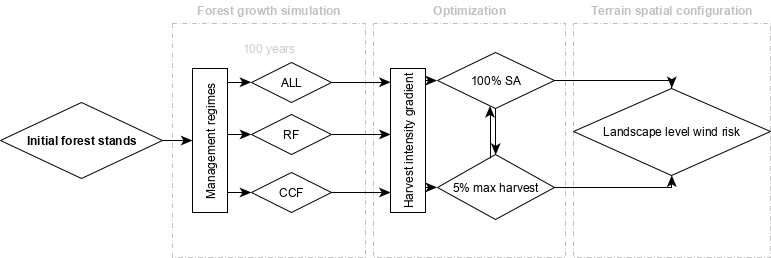
\includegraphics{/MyTemp/myGitLab/windDamage/externalFigs/overview2_horizontal.png}
\caption{The study workflow from collecting initial stand conditions
(2016) throught forest simulation growth under various ranges of forest
management, and constriuction of teh harvesting intensity gradient using
optimization to landscape level stand configurations.}
\end{figure}

\section{Methods}\label{methods}

\subsubsection{Study area}\label{study-area}

Our study area represents a typical Finnish production forested
landscape with relatively structurally homogenous forests stands. In
total we used 1475 forests stands aggregated within a single watershed
(number 14.534) in Central Finland, covering 2242 ha. Initial stand
conditions were collected as open source data from the Finnish Forest
Centre (available on www.metsaan.fi) providing currents stand conditions
in 2016.

Our input datasets includes initial stand conditions, simulation of the
forest regimes using forest growth simulator, and stand configurations
over the range of optimal landscape level forest management, varying
from over the harvest intensity is based on Eyvindosn et al. (2020)
study, please refer for more details.

\begin{figure}
\centering
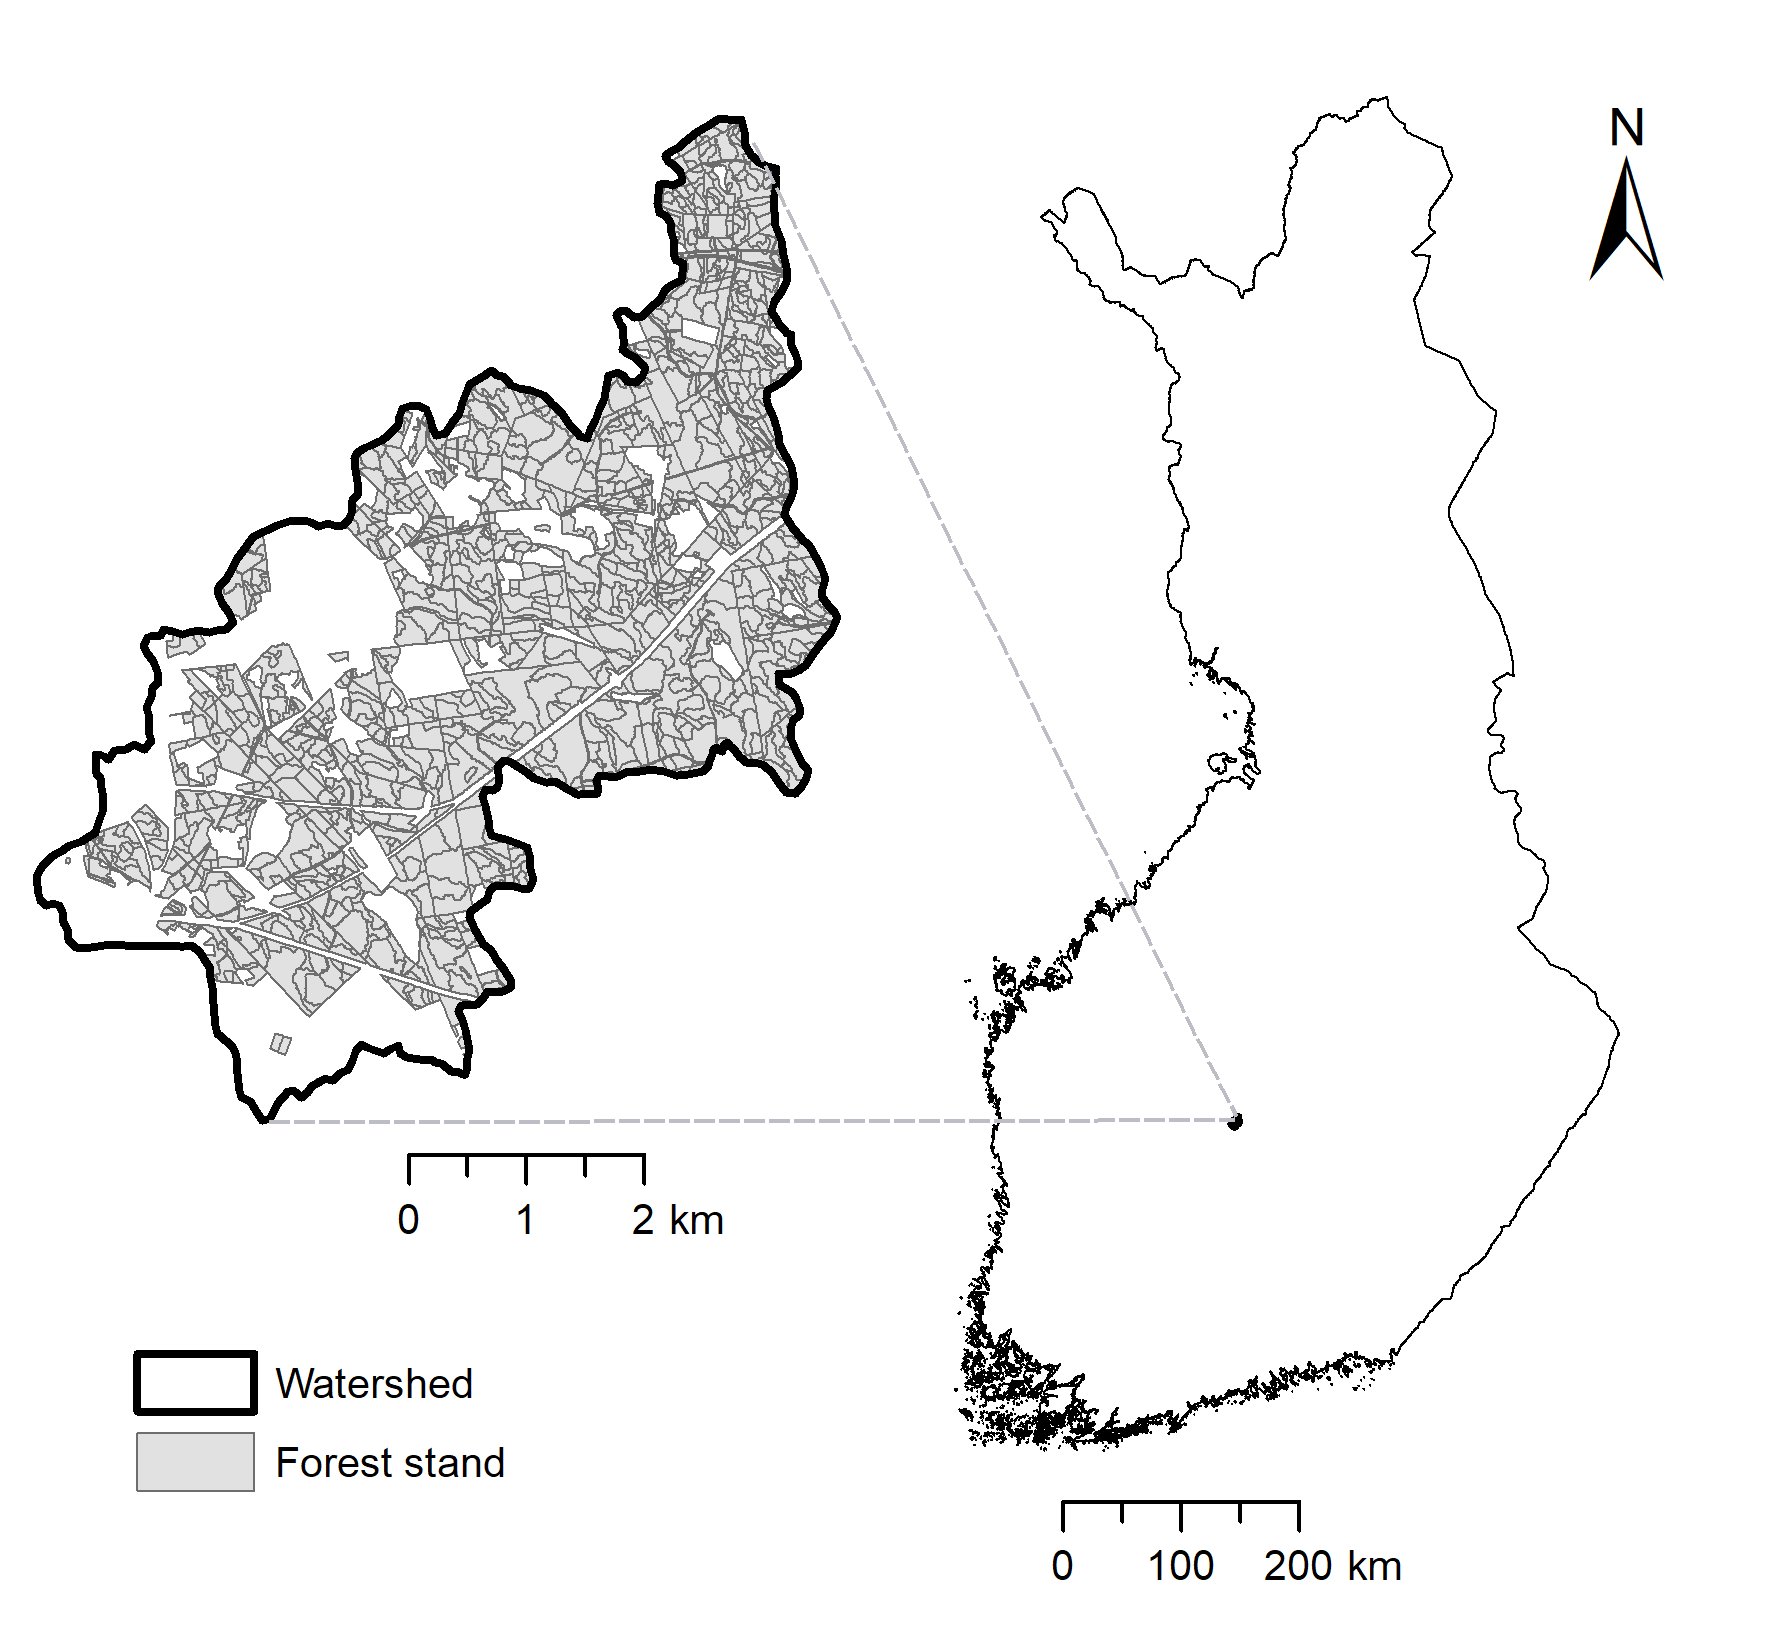
\includegraphics{/MyTemp/myGitLab/windDamage/externalFigs/studyArea_crop.png}
\caption{The study are located in Central Finland (watershed 14.534)
comprising 1475 forest stands.}
\end{figure}

\subsubsection{Forest stand development under different
regimes}\label{forest-stand-development-under-different-regimes}

We simulated the development of the forests stands using SIMO forest
growth simulator (Rasinmäki et al., 2009) over 100 years, separated into
20 5-year sequences. Each stand could be managed by up to 58 different
management regimes (the total number of regimes per stands depended on
the stand initial conditions), including 17 regimes for rotation
forestry (RF), 40 variations of continuous cover forest (CCF) and one
set aside (SA), where no management actions were taken. RF regimes
different in in timing of final felling, optionali thinning
(present/absent), and increase in retained green trees after final cut
(more details in Eyvindson et al., 2018). Basic CCF management follows
rules from Äijälä et al. (2014). To increase the range of CCF
managements, we varied two rules defining the timing of harvesting:
site-specific basal area and timing of the first thining. The
pre-defined site-specific basal area (m2/ha) requirement (16m2/ha for
less fertile sites to 22m2/ha for fertile sites) prior to harvesting was
modified by -3, ±0, +3, +6, and we delayed the timing of the first
harvest in 5 year increments up to a delay of 45 years.

\subsubsection{Optimization}\label{optimization}

The collection of the optimal management regimes explore the trade-offs
between between net present income (NPI) and forest multifunctionality.
NPI represents economic value of the forests estimated by Metsähallitus
(the Finnish governmental organization managing state owned forests) and
higher NPI value presents higher timber extraction and oppose the
proportion of the set-aside forest stands (i.e.~without active
harvesting). Optimization process over the NPI gradient was run using
only RF, only CCF management types, or all possible managements (RF and
CCF) included over the gradient of NPI values, from 0 (representing
set-aside or no management in all stands) maximal amount of extracted
timber (leaving up to 5\% of SA stands). The optimization process
resulted in creating of 63 alternative landscape development paths over
100 years period in 20 5-years time steps that different in applied
management types (3) and levels of timber extraction (21), further
referred as scenarios. Each optimized scenario represents a collection
of management regimes applied uniquely over every stand. This setup
allowed us to reconstruct the dynamics landscape development over time
under combination of management regimes, and harvest extraction
gradient.

\subsubsection{Wind risk calculation}\label{wind-risk-calculation}

We have calculated the probability of wind damage based on
({\textbf{???}}) binomial generalized linear model with logit-link
function for each stand, under each scenario and at every time step.
({\textbf{???}}) This model calculates the probability of the wind
damage considering available relevant open-access datasets, specifically
dominant tree species, dominant tree height, time since thinning,
predicted levels on max wind speed (for next 10 years, this remain
stable in this study), evaluated if stand has open edge, soil type,
mineral soil depth, site fertility and temperature sum (refer to
(Suvanto et al., 2019) for all details). As it is difficult to predict
specific location of the occurrence of strong winds in the future, the
model outputs show the relative differences between stands, damage can
be only partial to the stand. To process the datasets, calculate damage
probability models and visualize results we used (R Development Core
Team, 2019).

\subsubsection{Data processing}\label{data-processing}

We calculated the probability of wind damage based on stand level for
each stand, scenario and time intervals. First, we evaluated wind damage
probability on stand level, which we averaged over the scenarios to
allow comparison over the harvesting gradient, and application of RF,
CCF and all possible management types. We hypothesized that RF would
increase wind damage risk dues to increasing number of open edges while
CCF would lower wind risk over the landscape. Further, we hypothetize
that higher levels of timber extraction would increase wind risk.
Lastly, we hypothetized than increasing amount of set-aside stands, over
the landscape together with CCF management would increase wind damage
risk due to larger present timber volume, and due to more frequent
thinning activities. We investigated wind risk in terms of available
timber volume, specifically saw and log timber volume. Lastly, we
explored the trends of wind risk relevant to stands height, changes and
species compositions.

\section{Results}\label{results}

\subsubsection{Landscape level wind risk under management restriction
and harvest intensity
scenarios}\label{landscape-level-wind-risk-under-management-restriction-and-harvest-intensity-scenarios}

The set-aside landscape level management resulted at the same mean
landscape level risk for all management regimes (Fig. 2). However,
intensifying harvesting triggers different responses under groups of
management regimes and intensification of the timber extraction. Sole
use of the RF managements lowered the wind risk with increasing harvest
intensity. On the other hand, both ALL and CCF scenarios increased the
wind risk where CCF monotonically increased with increasing harvesting
rates, while ALL regimes have slightly humpened curve shape, culminating
around inteinsity of 7.5K by ha. The CCF increases monotonically while
maximal harvesting increase the wind risk by 25\% compared to completely
set-aside stands.

\begin{figure}
\centering
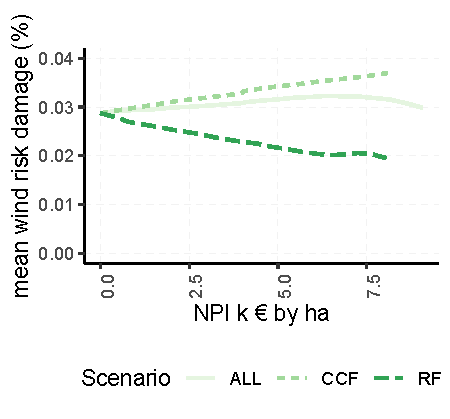
\includegraphics{test_manus_files/figure-latex/fig3_mean_risk_by_intensity_plot-1.pdf}
\caption{Mean wind risk damage for three types of management regimes
over harvest intensity gradient}
\end{figure}

\subsubsection{Timber volume at wind
risk}\label{timber-volume-at-wind-risk}

Increasing harvesting levels lowers the amount of the available timber
at any time step to be lost due to windthrows. Interestingly, the CCF
regimes produces higher logs volumes, while RF has higher production of
the pulp wood, which is in high demand by cheaper then log wood. The
same trends are visible for harvested log and pulp volumes. For ALL
management regimes, using all available management regimes, is located
between two extremities. The highest mean log timber volume as available
for the wind damage at lowest harvesting levels. Interestingly, under
RF, low levels of timber extraction increase levels of the pupl standing
volume. The highest amount of harvested log wood is produced by CCF
regimes, while RF dominates in harvesting pulp timber.

\begin{figure}
\centering
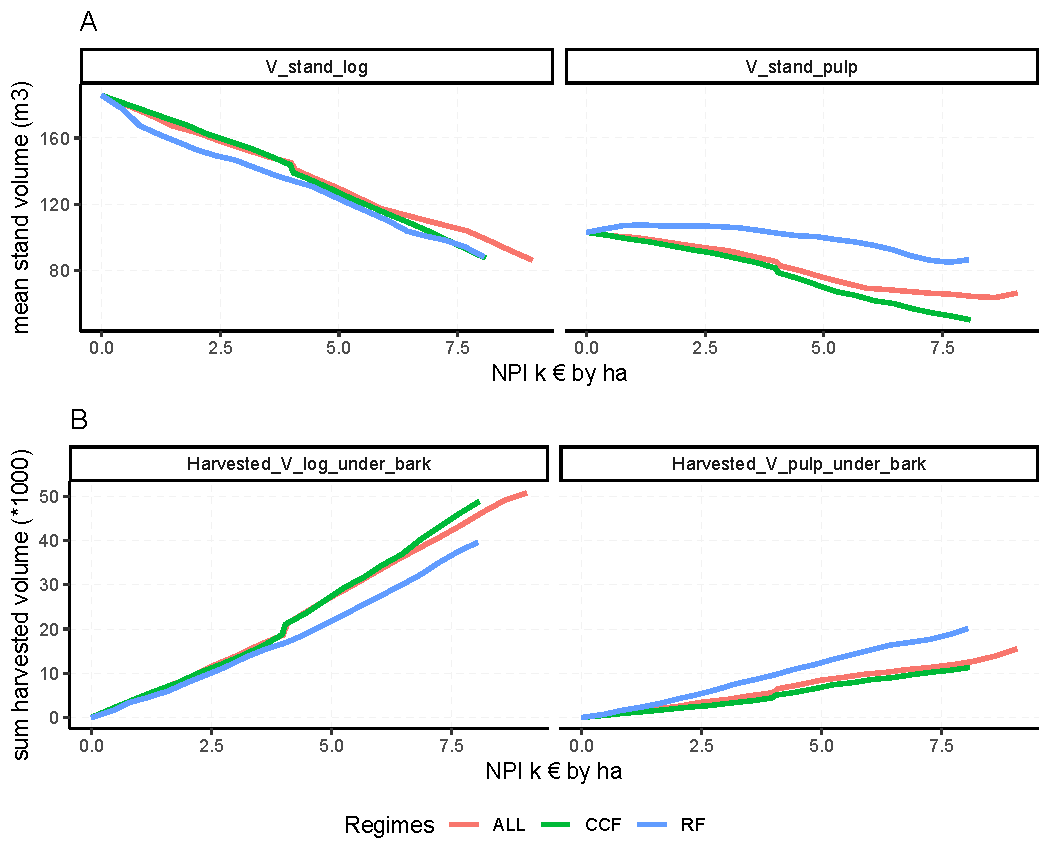
\includegraphics{test_manus_files/figure-latex/fig_4_plot_V_timber-1.pdf}
\caption{A. Mean standing and B. harvested pulp and log timber under
three types of management regimes over harvest intensity gradient}
\end{figure}

The intensification of the harvesting levels increases the proportion of
the pulp wood compared to log wood, especially in RF. In CCF, the
proportion among standing log and pulp volume remains at the same rate
(65:30) where the production of the log timber dominates See figure
@ref(fig:fig\_5\_proportion\_V\_pulp\_log).

\begin{figure}
\centering
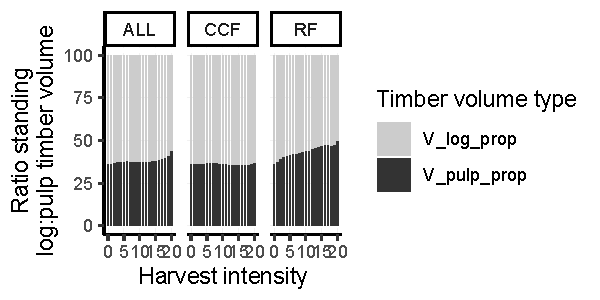
\includegraphics{test_manus_files/figure-latex/fig_5_proportion_V_pulp_log-1.pdf}
\caption{Ratio between standing log and pul volume (m\^{}3)}
\end{figure}

\subsubsection{Open stands frequency}\label{open-stands-frequency}

RF regimes increase the amount of stands with open edge with increasing
harvest intensity while CCF regimes maintain the same amount of open
stands over the harvest intensity gradient. Intensive RF increases
number of stands with open edge by 5\%.

\begin{figure}
\centering
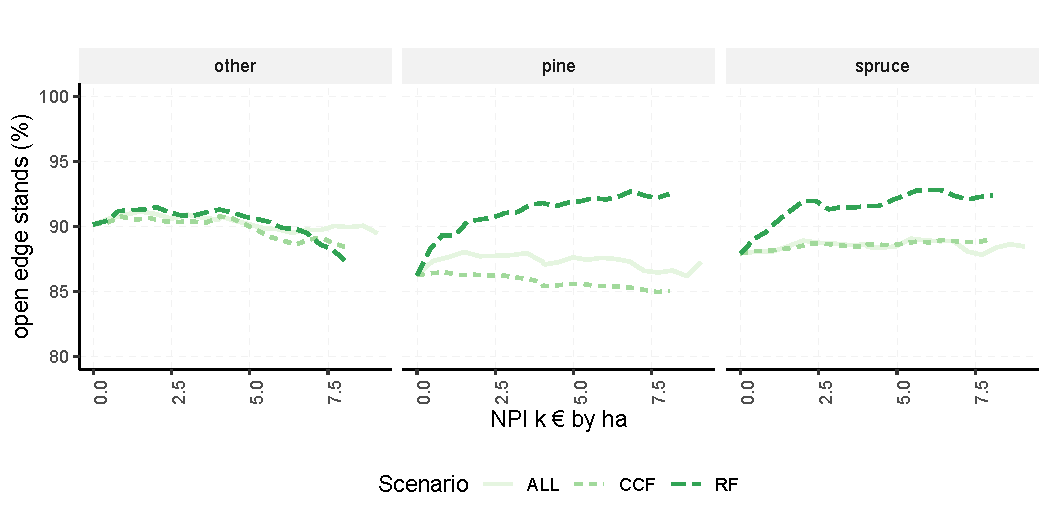
\includegraphics{test_manus_files/figure-latex/fig_6_count_open_edge-1.pdf}
\caption{Yearly count of stands with open edge over the intensity
gradient}
\end{figure}

\subsubsection{Changes in species
composition}\label{changes-in-species-composition}

\begin{figure}
\centering
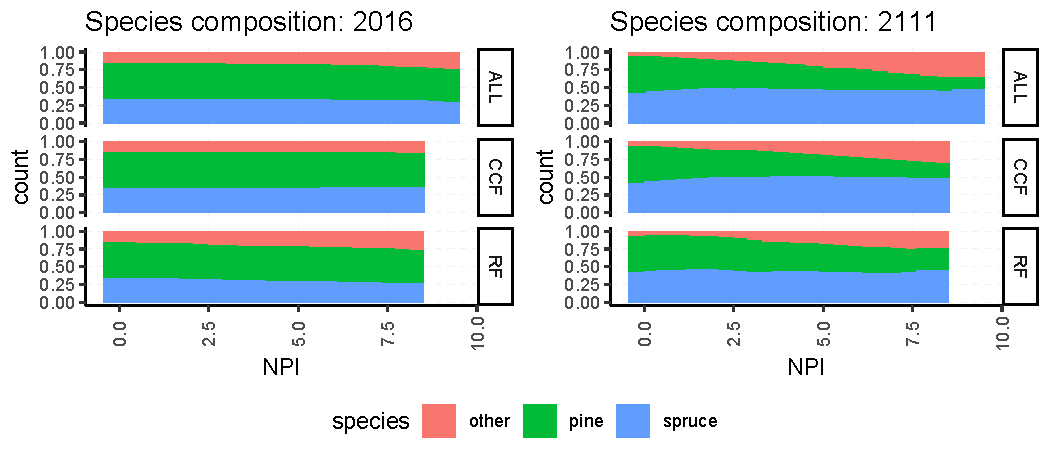
\includegraphics{test_manus_files/figure-latex/fig_7_species_change-1.pdf}
\caption{Changes in species composition under different management types
and harvest intensity}
\end{figure}

\section{Discussion}\label{discussion}

Should we discuss about findings?

\section{Close chunk}\label{close-chunk}

\section*{References}\label{references}
\addcontentsline{toc}{section}{References}


\end{document}


